\documentclass{article}

% if you need to pass options to natbib, use, e.g.:
%     \PassOptionsToPackage{numbers, compress}{natbib}
% before loading neurips_2019

% ready for submission
% \usepackage{neurips_2019}

% to compile a preprint version, e.g., for submission to arXiv, add add the
% [preprint] option:
%     \usepackage[preprint]{neurips_2019}

% to compile a camera-ready version, add the [final] option, e.g.:
\usepackage[final]{neurips_2019}

% to avoid loading the natbib package, add option nonatbib:
%     \usepackage[nonatbib]{neurips_2019}

\usepackage[utf8]{inputenc} % allow utf-8 input
\usepackage[T1]{fontenc}    % use 8-bit T1 fonts
\usepackage{hyperref}       % hyperlinks
\usepackage{url}            % simple URL typesetting
\usepackage{booktabs}       % professional-quality tables
\usepackage{amsfonts}       % blackboard math symbols
\usepackage{nicefrac}       % compact symbols for 1/2, etc.
\usepackage{microtype}      % microtypography
\usepackage{amsmath}        % because
\usepackage{graphicx}       % pictures
\usepackage{xcolor}         % colored text

% Macros
\newcommand{\blue}[1]{\textcolor{blue}{#1}}
\newcommand{\red}[1]{\textcolor{red}{#1}}

\title{}

% The \author macro works with any number of authors. There are two commands
% used to separate the names and addresses of multiple authors: \And and \AND.
%
% Using \And between authors leaves it to LaTeX to determine where to break the
% lines. Using \AND forces a line break at that point. So, if LaTeX puts 3 of 4
% authors names on the first line, and the last on the second line, try using
% \AND instead of \And before the third author name.

\author{%
  Mingcheng Wang, Eric Xia, Trevor Jung\\ % write a list of authors
  University of Washington \\
 \texttt{\{wmingch, ericxia, tjung2\}@uw.edu} \\ % write your email
}

\begin{document}

\maketitle
\bibliographystyle{unsrt}

% Template and style guide for the eproducibility project for CSE 517.

% Note that we slightly updated the style file for the CSE 517 project, so it is not exactly the same as 2020 ML Reproducibility Challenge (or later iterations).  In order to submit to a ML Reproducibility Challenge, please move the report to the official template, and get advice from the TA to make sure that your format is good.

\section*{\centering Reproducibility Summary}
%This summary section should be less than one page.

\subsection*{Scope of Reproducibility}
%State the main claim of the original paper you are trying to reproduce. We recommend picking the central claim of the paper.
We attempt to reproduce the claim that the authors’ decision-focused summarization model, \texttt{DecSum}, substantially outperforms text-only summarization methods and model-based
explanation methods in terms of decision faithfulness and representativeness.

\subsection*{Methodology}
%Briefly describe what you did and which resources did you use. E.g., did you use author's code, did you reimplement parts of the pipeline, how much time did it take to produce the results, what hardware you were using and how long it took to train/evaluate.
We used the author’s code, provided on \href{https://github.com/ChicagoHAI/decsum}{\blue{their Github}}. We download the Yelp dataset, provided freely on the
\href{https://www.yelp.com/dataset/download}{\blue{Yelp website}}. The author's scripts contain some code errors, and we fixed the code before it ran properly. All 15 simulations (7 were from paper
and other 8 were experiments beyond content of paper) are run over two Tesla V100 GPUs. Each simulation of DecSum took 14 hours to run, and training the Longformer took 4 hours.

\subsection*{Results}
%Start with your overall conclusion---where was your study successful and where not successful? Be specific and use precise language, e.g.,``we reproduced the accuracy to within 1\% of reported value, that upholds the paper's conclusion that it performs much better than baselines.'' Getting exactly the same number is in most cases infeasible, so you'll need to use your judgment to decide if your results support the original claim of the paper.
In line with the paper, DecSum outperforms the text-only summarization methods and model-based explanation methods in terms of decision faithfulness and representativeness. The additional experiments
indicate that the performance of DecSum is not sensitive to the model hyperparameters (e.g. max sequence length, summary length) and the training data used.

\subsection*{What was Easy}
%Describe which parts of your reproduction study were easy. E.g., was it easy to run the author's code, or easy to reimplement their method based on the description in the paper. The goal of this section is to summarize to the reader which parts of the original paper they could easily apply to their problem.
It was relatively easy to access the authors' code on Github and follow their repo's documentation. It was also easy to access and download the data used in the paper (the yelp dataset).

\subsection*{What was Difficult}
%Describe which parts of your reproduction study were difficult or took much more time than you expected. Perhaps the data was not available and you couldn't verify some experiments, or the author's code was broken and had to be debugged first. Or, perhaps some experiments just take too much time/resources to run and you couldn't verify them. The purpose of this section is to indicate to the reader which parts of the original paper are either difficult to reuse, or require a significant amount of work and resources to verify.
The author's scripts contain code errors and took some time to debug them. We also had limited computing resources and running all simulations took a lot more time than we expected. We were confused
by the authors' methodology in some parts of the paper, for example how sentences were chosen to compute decision representativeness, particularly for the diagram of the model prediction's PDF
on page 8 of the paper.

\subsection*{Communication with Original Authors}
%Briefly describe how much (if any contact) you had with the original authors.
We had no contact with the original authors.
\newpage

% Keep in mind that your page limit is 8, excluding references and the summary section above.
% For specific grading rubrics, please see the project instructions.

\section{Introduction}
%A  few  sentences  placing  the  work  in  context. Limit it to a few paragraphs at most; since your report is on reproducing a piece of work, you don’t have to motivate that work. However, it should be clear enough what the original paper is about and what its contributions are.
We attempt to reproduce the experiments described in the EMNLP 2021 paper \href{https://aclanthology.org/2021.emnlp-main.10.pdf}{\blue{Decision-Focused Summarization}} by Chao-Chun Hsu
and Chenhao Tan.~\cite{hsu-tan-2021-decision} This paper proposes a new technique called decision-focused summarization for the problem of text summarization. Traditionally, text summarization is done
only using textual information. However, this has issues. For instance, a common metric used to evaluate text summaries is non-redundancy, which encourages a summary to encompass a diverse range of
topics. But if a doctor wanted to analyze the risks of pancreatic cancer in a patient, it may not be useful to include information about a knee injury. Instead, with a decision-focused summarization
method, one could create summaries better tailored to a task. \\

The authors use the following setup: they leverage a supervised decision model, which takes as text as input and makes a decision. Then, the text summarization algorithm seeks to minimize loss on the
decision. The authors propose two new desiderata: decision faithfulness and decision representativeness. In addition, they also use textual non-redundancy as a third desiderata. \\

The authors find that decision-focused summarization outperforms text-only summarization methods and model-based explanation methods. In addition, they show that the decision-focused summarization
method outperforms other methods in aiding human decision-making in a challenging classification task.

\section{Scope of Reproducibility}
%Explain the claims from the paper you picked for the reproduction study and briefly motivate your choice. We recommend picking the claim that is the central contribution of the paper. To find what this contribution is, try to summarize the most important result of the paper in 1--2 sentences, e.g., ``This paper introduces a new activation function X that outperforms a similar activation function Y on tasks Z, V, and W.''
%Make the scope as specific as possible. It should be something that can be supported or rejected by your data. For example, this scope is too broad and lacks precise outcome (what is ``strong performance''?): ``Contextual embedding models have shown strong performance on a number of tasks across NLP. We will run experiments evaluating two types of contextual embedding models on datasets X, Y, and Z.''
%This scope is better because it's more specific and has an outcome that can be either supported or rejected based on your work: ``Finetuning pretrained BERT on SST-2 will have higher accuracy than an LSTM trained with GloVe embeddings.''
Parts we will be able to reproduce: \\
1.  Run DecSum and apply it to Yelp data set to find its performance, including the decision faithfulness and representativeness. \\
2. Compare the results of the above with the statistics provided in the paper. \\
3. Compare DecSum’s performance to text-only summarization and model-based explanation to see if DecSum indeed has better performance in terms of decision faithfulness and representativeness. \\

Parts we will not be able to reproduce: \\
1. The paper runs text-only summarization baselines (e.g., PreSumm, BART, Random) and model-based explanations (e.g. Integrated Gradients and Attention) to compare them with DecSum.
Given our time and computing resources, we may rely on the results of text-only summarization baselines and Model-based explanations shown in the paper, instead of running those simulations by ourselves. \\
2. The paper implemented the human evaluation by using Amazon Mechanical Turk to solicit human guesses on which restaurants would be rated higher after participants. We are not able to implement such
a high-scale data collection method like Amazon Mechanical Turk.

\subsection{Addressed Claims from the Original Paper}

We are testing the claim from the paper that DecSum substantially outperforms text-only summarization methods and model-based explanation methods in terms of decision faithfulness and representativeness.

\section{Methodology}
%This section is to explain your approach---did you use the author's code, did you aim to reimplement the approach from the paper description? Summarize the resources (code, documentation, GPUs) that you used.

\subsection{Model Descriptions}
%Describe the models used in the original paper, including the architecture, learning objective and the number of parameters.
The goal is to determine the most relevant information from a text for a particular decision to ultimately be a summary of sorts of human decision-making for a use-case. More formally, given an
input text $X = \{x_s\}_{s=1}^{S=1}$, where $S$ is the number of sentences, we wish to select a subset of sentences $\tilde{X}\subset X$ to support making a decision $y$. Thus, the training set,
$D_{train} = \{(X_i, y_i)\}$, will be processed in such a way as to find defining traits in a text that lead to a certain decision $y$. The yelp datset is then defined as follows: for each restaurant,
define $X$ to be the text body of the first $k$ reviews and let $y$ be the average ranking of the first $t$ reviews, where $t > k$ s.t. the problem is to predict future ratings.
Here, the parameters are $k$ and $t$; the researchers used $k = 10, t = 50$ s.t. their objective was to choose sentences amongst a restaurant’s first 10 reviews that supported predicting its future
review rating after 50 reviews.

\subsubsection{The Loss Function}
Loss functions were formalized from the need for the model to satisfy "decision faithfulness, decision representativeness, and textual non-redundancy", where $f:X\to y$ is the model's function. \\

\textbf{Decision faithfulness $\mathcal{L}_F$.} The sentences selected by the model should lead to the same decisions as the full input text: for selected sentences $\tilde{X}\subset X$, we want
$f(\tilde{X})\simeq f(X)$. We take the loss function to be the log absolute difference between $f(\tilde{X})$ and $f(X)$. \\
\textbf{Decision representativeness $\mathcal{L}_R$.} We want the summary of the decision distribution outputted by the model, $\hat{Y}_{\tilde{X}} = \{f(x)\mid x\in\tilde{X}\}$, to be close to the decision
distribution of all sentences from the full text, $\hat{Y}_X = \{f(x)\mid x \in X\}$. Thus, we take $\mathcal{L}_R$ to be the log Wasserstein distance between $\hat{Y}_{\tilde{X}}$ and
$\hat{Y}_{X}$. \\
\textbf{Textual non-redundancy $\mathcal{L}_D$.} As the model's objective is a summary of the reasoning for the writer's decision, we use cosine similarity to encourage dissimilar sentences in the
output summary. \\

\abovedisplayskip=0pt
\textbf{Final loss function.} Combining these three, out loss function is

\begin{align*}
    \mathcal{L}(\tilde{X}, X, f)    &= \alpha\mathcal{L}_F (\tilde{X}, X, f) + \beta\mathcal{L}_R (\tilde{X}, X, f) + \gamma\mathcal{L}_D (\tilde{X}) \\
                                    &= \alpha\log{|f(\tilde{X}) - f(X)|} + \beta\log{(W(\hat{Y}_{\tilde{X}}, \hat{Y}_X))}
                                    + \gamma\sum_{x\in\tilde{X}}\substack{\text{max}\\ x'\in \tilde{X} - \{x\}} \text{cossim}(s(x), s(x')),
\end{align*}
\belowdisplayskip=0pt

where $\alpha, \beta, \gamma$ are hyperparameters that determine the weight of each component of the loss function.

\subsubsection{The Model}
DecSum is an iterative algorithm that greedily selects a sentence that minimizes the loss function: In order to select $K$ sentences from an input $X$, in each step $k=\{1, \dots, K\}$, iteratively
choose a sentence from the remaining sentences $\hat{x}\in X - \tilde{X}_{k-1}$ that achieves the lowest loss $\mathcal{L}(\tilde{X}_{k-1}\cup \{\hat{x}\}, X, f)$ where $\tilde{X}_{k-1}$ is the current
summary using $k-1$ sentences. When $\beta$ is positive, only $\mathcal{L}_R$ is used in the first step "to encourage the algorithm to explore the full distribution rather than stalling at the sentence
most faithful to $f(X)$". In practice, beam search with beam search size 4 was used to improve the greedy algorithm.

A 64\%/16\%/20\% training/validation/test set split was employed, and Longformer~\cite{beltagy2020longformer} (\href{https://github.com/allenai/longformer}{Github code here}) was used to fine-tune the
regression models.

\begin{figure}[!ht]
    \centering
    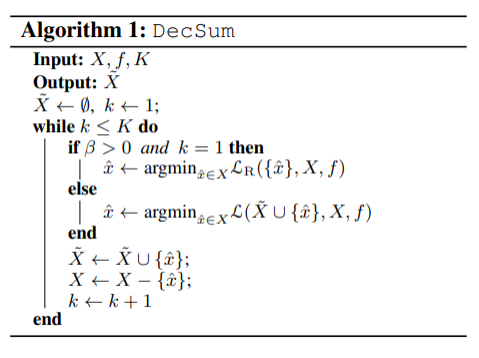
\includegraphics[scale=1]{../assets/DecSum_Algo}
    \caption{DecSum Algorithm}
    \label{fig:1}
\end{figure}



\subsection{Dataset Description and Code}
% Describe the datasets you used and how you obtained them.
% Describe whether you use the existing code or write your own code, with the link to the code and which languange/packages were used. Note that the github repo you link should be public and have a clear documentation.
We use the author’s code, provided on \href{https://github.com/ChicagoHAI/decsum}{\blue{their Github}}. After cloning the repo and creating a conda environment with Python 3.7,
dependencies may be installed through the repo's instructions under the "Env" heading, no modifications needed. We used the Yelp dataset, provided freely on the
\href{https://www.yelp.com/dataset/download}{\blue{Yelp website}}, and when uncompressed, is a directory of json files in the format \texttt{yelp\_academic\_dataset\_CATEGORY.json}. \\

For the author's preprocessing instructions on their repo to work, we made the following modifications: \\
$\bullet$ Changed the format of all the json files to \texttt{CATEGORY.json} instead \\
$\bullet$ Line 24 of \texttt{preprocess/yelp\_preprocess.py} was changed from \texttt{int(datetime(strptime()))} to \texttt{int(datetime.datetime(strptime()))} \\
$\bullet$ Made new directory \texttt{OUTPUT\_DIR} \\

The preprocessing script effectively reads in the 52268 restaurants and associated reviews from the dataset and computes the average of the first 50 reviews. The dataset split used is
64\%/16\%/20\% train/valid/test, so in terms of restaurants, 33452/8363/10453. \\

For training the Longformer model, one has to run the command in the repo with sudo, after changing \texttt{OUTPUT\_DIR}, \texttt{YELP\_OUTPUT\_DIR}, \texttt{CAHCE\_DIR} to
\texttt{OUTPUT\_DIR/transformers}, \texttt{OUTPUT\_DIR}, \texttt{OUTPUT\_DIR/transformers\_cache} respectively, in \texttt{train\_transformer.sh}. \\

For running DecSum, go to \texttt{sentence\_select.sh} and change \texttt{OUTPUT\_DIR} to \texttt{OUTPUT\_DIR} and \texttt{MODEL\_PATH} to the path of \texttt{epoch=2-val\_loss=0.14.ckpt}. Similarly,
correct the paths of \texttt{OUTPUT\_DIR} and \texttt{MODEL\_PATH} in \texttt{single\_sentence\_score.sh} before running it to get the decision scores for individual sentences. \\

To get the Wasserstein distance between the predictions using full reviews and summaries generated by DecSum, first uncomment the bottom python command in \texttt{single\_sentence\_score.sh}, and then
comment the top command. Run \texttt{bash scripts/single\_sentence\_score.sh} and then \texttt{python wasserstein.py} from our \href{https://github.com/ericxiaseattle/CSE517-Project}{Github} repo,
in which the above errors are also fixed. \\

The additional experiments we took beyond the scope of the paper may be run by modifying the parameters in \texttt{sentence\_select.sh} (e.g. \texttt{num\_sentences}, \texttt{num\_review}) and
\texttt{train\_transformer.sh} (e.g. \texttt{max\_seq\_length}). The script that generates the pdf plot in our reproduction of the paper may also be found on our repo, and can be run with
\texttt{python pdf.py}.

\subsection{Hyperparameters}
%Describe how you set the hyperparameters and what was the source for their value (e.g., paper, code, or your guess).

Longformer takes 102M parameters with half precision and makes use of the Huggingface transformers package~\cite{wolf-etal-2020-transformers} and the
AdamW optimizer~\cite{DBLP:journals/corr/abs-1711-05101}, with learning rate $5\cdot 10^{-5}$ and a linear warmup of 500 steps for the learning rate. The model is trained for 3 epochs where
the batch size is 4 and the maximum input token length is 3,000. There are 12 hidden layers, each of size 768, and there are 12 attention heads with attention window 512. The dropout is 0.1. \\

One hyperparameter group we used was what values to use for the three desiderata (decision faithfulness, decision representativeness, textual non-redundancy) when implementing DecSum, i.e.
what values in $\{0,1\}$ to use for the DecSum hyperparameter group $(\alpha, \beta, \gamma)$.
We ran our experiments using the same as the ones given in Table 1 of their paper.

\subsection{Experimental Setup and Computational Requirements}
%Explain how you ran your experiments, e.g. the CPU/GPU resources and provide the link to your code and notebooks.
%Provide information on computational requirements for each of your experiments. For example, the number of CPU/GPU hours and memory requirements.
%Mention both of your estimation before running the experiments and actual resources took for reproducing the experiments.
%You'll need to think about this ahead of time, and write your code in a way that captures this information so you can later add it to this section.
The authors preprocess their data and train their model on a single RTX 3090 setup. The performance of Tesla V100s lags behind an RTX 3090, so we expect that time spent on
training and processing the data to be noticeably more than that of the authors. For reference, the authors spent an hour per epoch on fine-tuning the regression models with Longformer
before DecSum was ran, and less than an hour on DecSum itself for every trial.
Perhaps only 8 GB RAM is necessary, as the yelp dataset itself is only 13 GB.
Similarly, the disk memory usage should thus be slightly above 13 GB, perhaps around 14 GB.
Using a 2xTesla V100 GPU setup, we estimate the runtime of Longformer to be 4 hours and maximum 4 hours for DecSum for every $(\alpha, \beta, \gamma)$ permutation of the trial as well. \\

In reality, training Longformer took 4/3 hours for each of its 3 epochs, for a total of 4 hours. For DecSum, each trial took much longer than expected, for a total of 14 hours—10 hours for training
and 4 hours for the prediction and evaluation on the test set.
There were a total of 15 trials we ran, 7 of which were in the paper and 8 that were additional experiments we took beyond the scope of the paper to see
the effect of certain hyperparameters. Initially, we tried running the models with 8 GB of RAM, however this led to it crashing, so we ultimately used 16 GB of RAM to run the experiments instead.
We used ~15 GB of disk memory: 13 GB from the yelp dataset and the rest from the transformer and pretrained models used in the scripts wrote by the authors in the pipeline.

\section{Results}
%Start with a high-level overview of your results. Does your work support the claims you listed in section \ref{claims}? Keep this section as factual and precise as possible, reserve your judgment and discussion points for the ``Discussion'' section that comes later.
%Go into each individual result you have, say how it relates to one of the claims and explain what your result is. Logically group related results into sections. Clearly state if you have gone beyond the original paper to run additional experiments and how they relate to the original claims.
%Tip 1: Be specific and use precise language, e.g. ``we reproduced the accuracy to within 1\% of reported value; that upholds the paper's conclusion that it performs much better than baselines.'' Getting exactly the same number is in most cases infeasible, so you'll need to use your judgment to decide if your results support the original claim of the paper.
%Tip 2: You may want to use tables and figures to demonstrate your results.
% The number of subsections for results should be the same as the number of hypotheses you are trying to verify.

\subsection{Result of Reproducing Experiments in Paper}

We are only testing the first and only claim:
that DecSum substantially outperforms text-only summarization methods and model-based explanation methods in terms of decision faithfulness and representativeness.

\subsubsection{Decision Faithfulness}
We are able to get similar results as the authors did, and the claim being tested was indeed true for us as well.
As shown in Table 1, MSE of DecSum (1,1,1) is quite close to the result using all texts, and much better as compared to the Text-only summarization
method and model-based explanation methods. Consistent with the paper, out of three hyperparameters of DecSum, the hyperparameter of decision faithfulness is the most important one for the MSE metric,
while two other hyperparameters have less impact on the MSE of the results. \\

Note that in our DecSum experiments, (0,1,0) has the worst model performance, with MSE of 0.5718. The paper, however, shows the DecSum experiment (0,0,1) has the worst model performance,
with an MSE of 0.565. This may be related to model randomness. It may also show that decision representativeness and textual non-redundancy by themselves are not good and consistent metrics for
generating summaries for decision tasks.

\begin{table}[ht]
    \centering
    \caption{MSE of Model Predictions Based on Summaries of Different Methods}
    \begin{tabular}{|c|c|}
        \hline \textbf{Method} & \textbf{MSE} \\
        \hline All & 0.1336 \\
        \hline Text-only summarization method - random & 0.475 \\
        \hline Text-only summarization method - BART & 0.502 \\
        \hline Text-only summarization method - PreSumm & 0.478 \\
        \hline Model-based explanation methods - IG & 0.565 \\
        \hline Model-based explanation methods - Attention & 0.715 \\
        \hline DecSum (1,1,1)   & 0.1338 \\
        \hline DecSum (1,1,0)   & 0.1336 \\
        \hline DecSum (1,0,1)   & 0.1339 \\
        \hline DecSum (0,1,1)   & 0.3196 \\
        \hline DecSum (1,0,0)   & 0.1336 \\
        \hline DecSum (0,1,0)   & 0.5718 \\
        \hline DecSum (0,0,1)   & 0.2362 \\ \hline
    \end{tabular}
\end{table}



\subsubsection{Decision Representativeness}
Table 2 shows the Wasserstein distance between model predictions of the selected sentences with those of all the sentences. In line with the paper, DecSum has much lower values of Wasserstein distance
(i.e., better decision representativeness) than the text-only summarization method and model-based explanation methods.

\begin{table}[ht]
    \centering
    \caption{Wasserstein Distance Between Model Predictions of the Selected Sentences With Those of All the Sentences} \\
    \begin{tabular}{|c|c|}
        \hline \textbf{Method} & \textbf{Wasserstein Distance} \\
        \hline Text-only summarization method - random & 0.398 \\
        \hline Text-only summarization method - BART & 0.423 \\
        \hline Text-only summarization method - PreSumm & 0.412 \\
        \hline Model-based explanation methods - IG & 0.62 \\
        \hline Model-based explanation methods - Attention & 0.64 \\
        \hline DecSum (1,1,1)   & 0.06525 \\
        \hline DecSum (1,1,0)   & 0.38331 \\
        \hline DecSum (1,0,1)   & 0.00048 \\
        \hline DecSum (0,1,1)   & 0.00257 \\
        \hline DecSum (1,0,0)   & 0.00047 \\
        \hline DecSum (0,1,0)   & 0.00257 \\
        \hline DecSum (0,0,1)   & 0.14236 \\ \hline
    \end{tabular}
\end{table}

Following the paper, we plot the density distribution of model predictions to investigate model decision representativeness. Figure 2 shows the result for one selected restaurant.
As shown in Figure 2, the DecSum is able to capture a sentence with a low predicted rating from reviews of IHOP, while PreSumm predicts ratings all above 3.
Such a result also indicates DecSum has better decision representativeness, as compared to other summary methods  (i.e. Text-only summarization and Model-based explanation methods).
Dots on the plot represent selected sentences on the distribution of model predictions. Please note that in our pdf plot we arbitrarily chose the sentences to be represented by the circles and stars,
as we did not understand how the authors chose their selected sentences in their density distribution plot from the paper.

\begin{figure}[!ht]
    \centering
    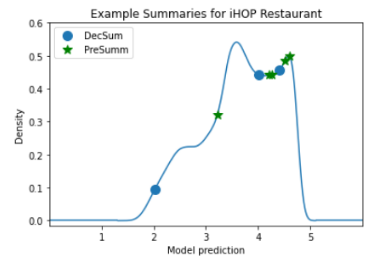
\includegraphics[scale = 0.8]{../assets/PDF}
    \caption{Example PreSumm and DecSum Summaries for the iHOP restaurant}
    \label{fig:2}
\end{figure}

\pagebreak
\subsection{Additional Results not Present in the Original Paper}
%Describe any additional experiments beyond the original paper. This could include experimenting with additional datasets, exploring different methods, running more ablations, or tuning the hyperparameters. For each additional experiment, clearly describe which experiment you conducted, its result, and discussion (e.g., what is the indication of the result).
In this subsection, we document the additional experiments we have carried out to investigate the sensitivity of DecSum's performance to the hyperparameters.

\subsubsection{Data Related - Training Data Size}
In the original paper, \%64 of the yelp dataset is used to train the model. Here, we tried halving the training data size to see its impact. As Table 3 shows, halving the training data only decreases
the performance by a bit as compared to the result using the full training data.

\begin{table}[ht]
    \centering
    \caption{MSE of Model Predictions for [Default, Half] Training Data Size}
    \begin{tabular}{|c|c|}
        \hline \textbf{Experiments} & \textbf{MSE} \\
        \hline DecSum (1,1,1) with default training data & 0.1338 \\
        \hline DecSum (1,1,1) with half of training data & 0.2246 \\ \hline
    \end{tabular}
\end{table}

\subsubsection{Data Related - Number of Reviews for Computing Average Rating}
In the original paper, the authors choose 50 as the number of reviews for computing average rating. Here we tried 30 and 70 as the number of reviews for computing average rating to see its impact.
As expected, using a smaller number of reviews could improve the model performance, but as indicated in Table 4, the performance of DecSum is not sensitive to this hyperparameter.

\begin{table}[ht]
    \centering
    \caption{MSE of Model Predictions with [default, 30, 70] Reviews}
    \begin{tabular}{|c|c|}
        \hline \textbf{Method} & \textbf{MSE} \\
        \hline DecSum (1,1,1) with 50 reviews (default) & 0.1338 \\
        \hline DecSum (1,1,1) with 30 reviews & 0.1186 \\
        \hline DecSum (1,1,1) with 70 reviews & 0.1369 \\ \hline
    \end{tabular}
\end{table}

\subsubsection{Transformer Related - Max Sequence Length}

The authors choose 3000 as the max sequence length when training the Longformer. Here we tried 1000 and 4000 as the max sequence length to see its impact. We could see the performance is much worse
if we use the max sequence length 4000 for Longformer, which may be because it takes more epochs to converge for the longer sequence length.
While if we choose the 1000 max sequence length for Longformer, the performance decreases only a bit.

\begin{table}[ht]
    \centering
    \caption{MSE of Model Predictions for [default, 1000, 4000] Max Sequence Length for Longformer}
    \begin{tabular}{|c|c|}
        \hline \textbf{Experiments} & \textbf{MSE} \\
        \hline DecSum (1,1,1) with max seq length 3000 (default) & 0.1338 \\
        \hline DecSum (1,1,1) with max seq length 1000 & 0.1456 \\
        \hline DecSum (1,1,1) with max seq length 4000 & 0.3926 \\ \hline
    \end{tabular}
\end{table}

\subsubsection{DecSum Related - Summary Length}

In the paper, the authors choose 50 tokens as the summary length. Here we also tried using 10, 30, 70 tokens as the summary length to see its impact on the prediction results.
As shown in Table 6, the model with higher summary length tends to have better prediction (lower MSE and higher accuracy).
Such results are in our expectations, given that with a longer summary length, less information has been truncated and thus the model is able to make better predictions.
But the impact of summary length is generally small and may not be statistically significant.
Note that, using 70 summary length, the training time is about 1.5 times of the default version (i.e., 50 summary length).

\begin{table}[ht]
    \centering
    \caption{MSE of Model Predictions for [default, 30, 70] Summary Length}
    \begin{tabular}{|c|c|}
        \hline \textbf{Experiments} & MSE \\
        \hline DecSum (1,1,1) with 50 summary length (default) & 0.1338 \\
        \hline DecSum (1,1,1) with 30 summary length & 0.1365 \\
        \hline DecSum (1,1,1) with 70 summary length & 0.1335 \\ \hline
    \end{tabular}
\end{table}



\section{Discussion}
%Describe larger implications of the experimental results, whether the original paper was reproducible, and if it wasn’t, what factors you believe made it irreproducible.
%Give your judgment on whether  the evidence you got from your experiments supports the claims of the paper. Discuss the strengths and weaknesses of your approach---perhaps you didn't have time to run all the experiments, or perhaps you did additional experiments that further strengthened the claims in the paper.
Generally, we are able to reproduce the paper result. As Table 1 shows, the results of different model simulations run by ourselves are close to the paper’s result, and shows that DecSum outperforms
the text-only summarization methods and model-based explanation methods in decision faithfulness and representativeness.

\subsection{What was Easy}
%Describe which parts of your reproduction study were easy. E.g., was it easy to run the author's code, or easy to reimplement their method based on the description in the paper. The goal of this section is to summarize to the reader which parts of the original paper they could easily apply to their problem.
%Tip: Be careful not to give sweeping generalizations. Something that is easy for you might be difficult to others. Put what was easy in context and explain why it was easy (e.g., code had extensive API documentation and a lot of examples that matched experiments in papers).
The authors have uploaded their code in the Github, and the instructions to run the codes are clear. Therefore, it is relatively easy for us to run the experiments and reproduce the paper’s results.
The data (i.e., Yelp dataset) used in the paper is open-access and so we were able to easily obtain the required data for the experiments.

\subsection{What was Difficult}
%Describe which parts of your reproduction study were difficult or took much more time than you expected. Perhaps the data was not available and you couldn't verify some experiments, or the author's code was broken and had to be debugged first. Or, perhaps some experiments just take too much time/resources to run and you couldn't verify them. The purpose of this section is to indicate to the reader which parts of the original paper are either difficult to reuse, or require a significant amount of work and resources to verify.
%Tip: Be careful to put your discussion in context. For example, don't say ``the math was difficult to follow,'' say ``the math requires advanced knowledge of calculus to follow.''
In the paper’s Github page, the csv files under the directory of preprocess are incorrect.
At the beginning of the project, it took us some time to figure out the particular bugs in the authors' code. The authors also used human evaluation (i.e. crowdsourcing human evaluation of model
predictions using Amazon Mechanical Turk) in their paper to test the performance of DecSum, but it was not possible for us to employ this type of evaluation in our reproduction of the paper. Each
DecSum trial took around 14 hours to run. In order to reproduce the paper’s result, we have carried out more than 15 DecSum experiments, which took much time given the limited computing resources we
had.

\subsection{Recommendations for Reproducibility}
%Describe a set of recommendations to the original authors or others who work in this area for improving reproducibility.
The scripts provided on the repo had code errors that we had to fix before it ran properly. The GitHub documentation was incomplete
(the README.md is empty for sections “Baseline methods” and “Generating Experiment Plots”). The heatmap in the paper and the pdf were hard to interpret and therefore not ideal when we were trying to
replicate them.

\section*{Communication with Original Authors}
%Document the extent of (or lack of) communication with the original authors. To make sure the reproducibility report is a fair assessment of the original research we recommend getting in touch with the original authors. You can ask authors specific questions, or if you don't have any questions you can send them the full report to get their feedback.
We had no correspondence with the original authors.


\bibliography{projectv2}

\end{document}
